\documentclass[e4_tp1_main.tex]{subfiles}

\begin{document}

\section{Ejercicio 3}

Se procedi\'o a integrar lo desarrollado en el ejercicio 1 con el ejercicio 2, switcheando la fuente buck con el circuito de disparo estudiado. 

En la figura \ref{fig:curvas3} observamos c\'omo la presencia del switch ``real'' afecta variables internas de la fuente. En primer lugar, los tiempos de conmutaci\'on del MOS son visibles en el gr\'afico, en comparaci\'on con la curva ideal. Sus efectos se ven claramente en el resto de las curvas: en $v_L$ se observa que le duty efectivo obtenido es superior a cuando se utiliz\'o el switch ideal. En efecto, la salida en este caso es de $V_O\simeq3.71V$, lo cual es consistente con tener un duty mayor.

A su vez, esto provoca que la corriente de la bobina tenga pendiente positiva por m\'as tiempo, lo cual explica el delay que se observa entre las curvas con llave ideal y real. Se observa tambi\'en que la corriente media es mayor con la llave real, lo cual es consistente con tener una tensi\'on de salida, y por lo tanto una corriente de salida, mayor.

En cuanto al diodo, volvemos a observar que conmuta m\'as tarde por el aumento del duty, pero adem\'as en este caso los picos de inversa son acotados: llegan a un m\'aximo de $I_{rr}=1.84$A.

\begin{landscape}
	\vspace*{\fill}
	\begin{figure}[ht]
		\centering
		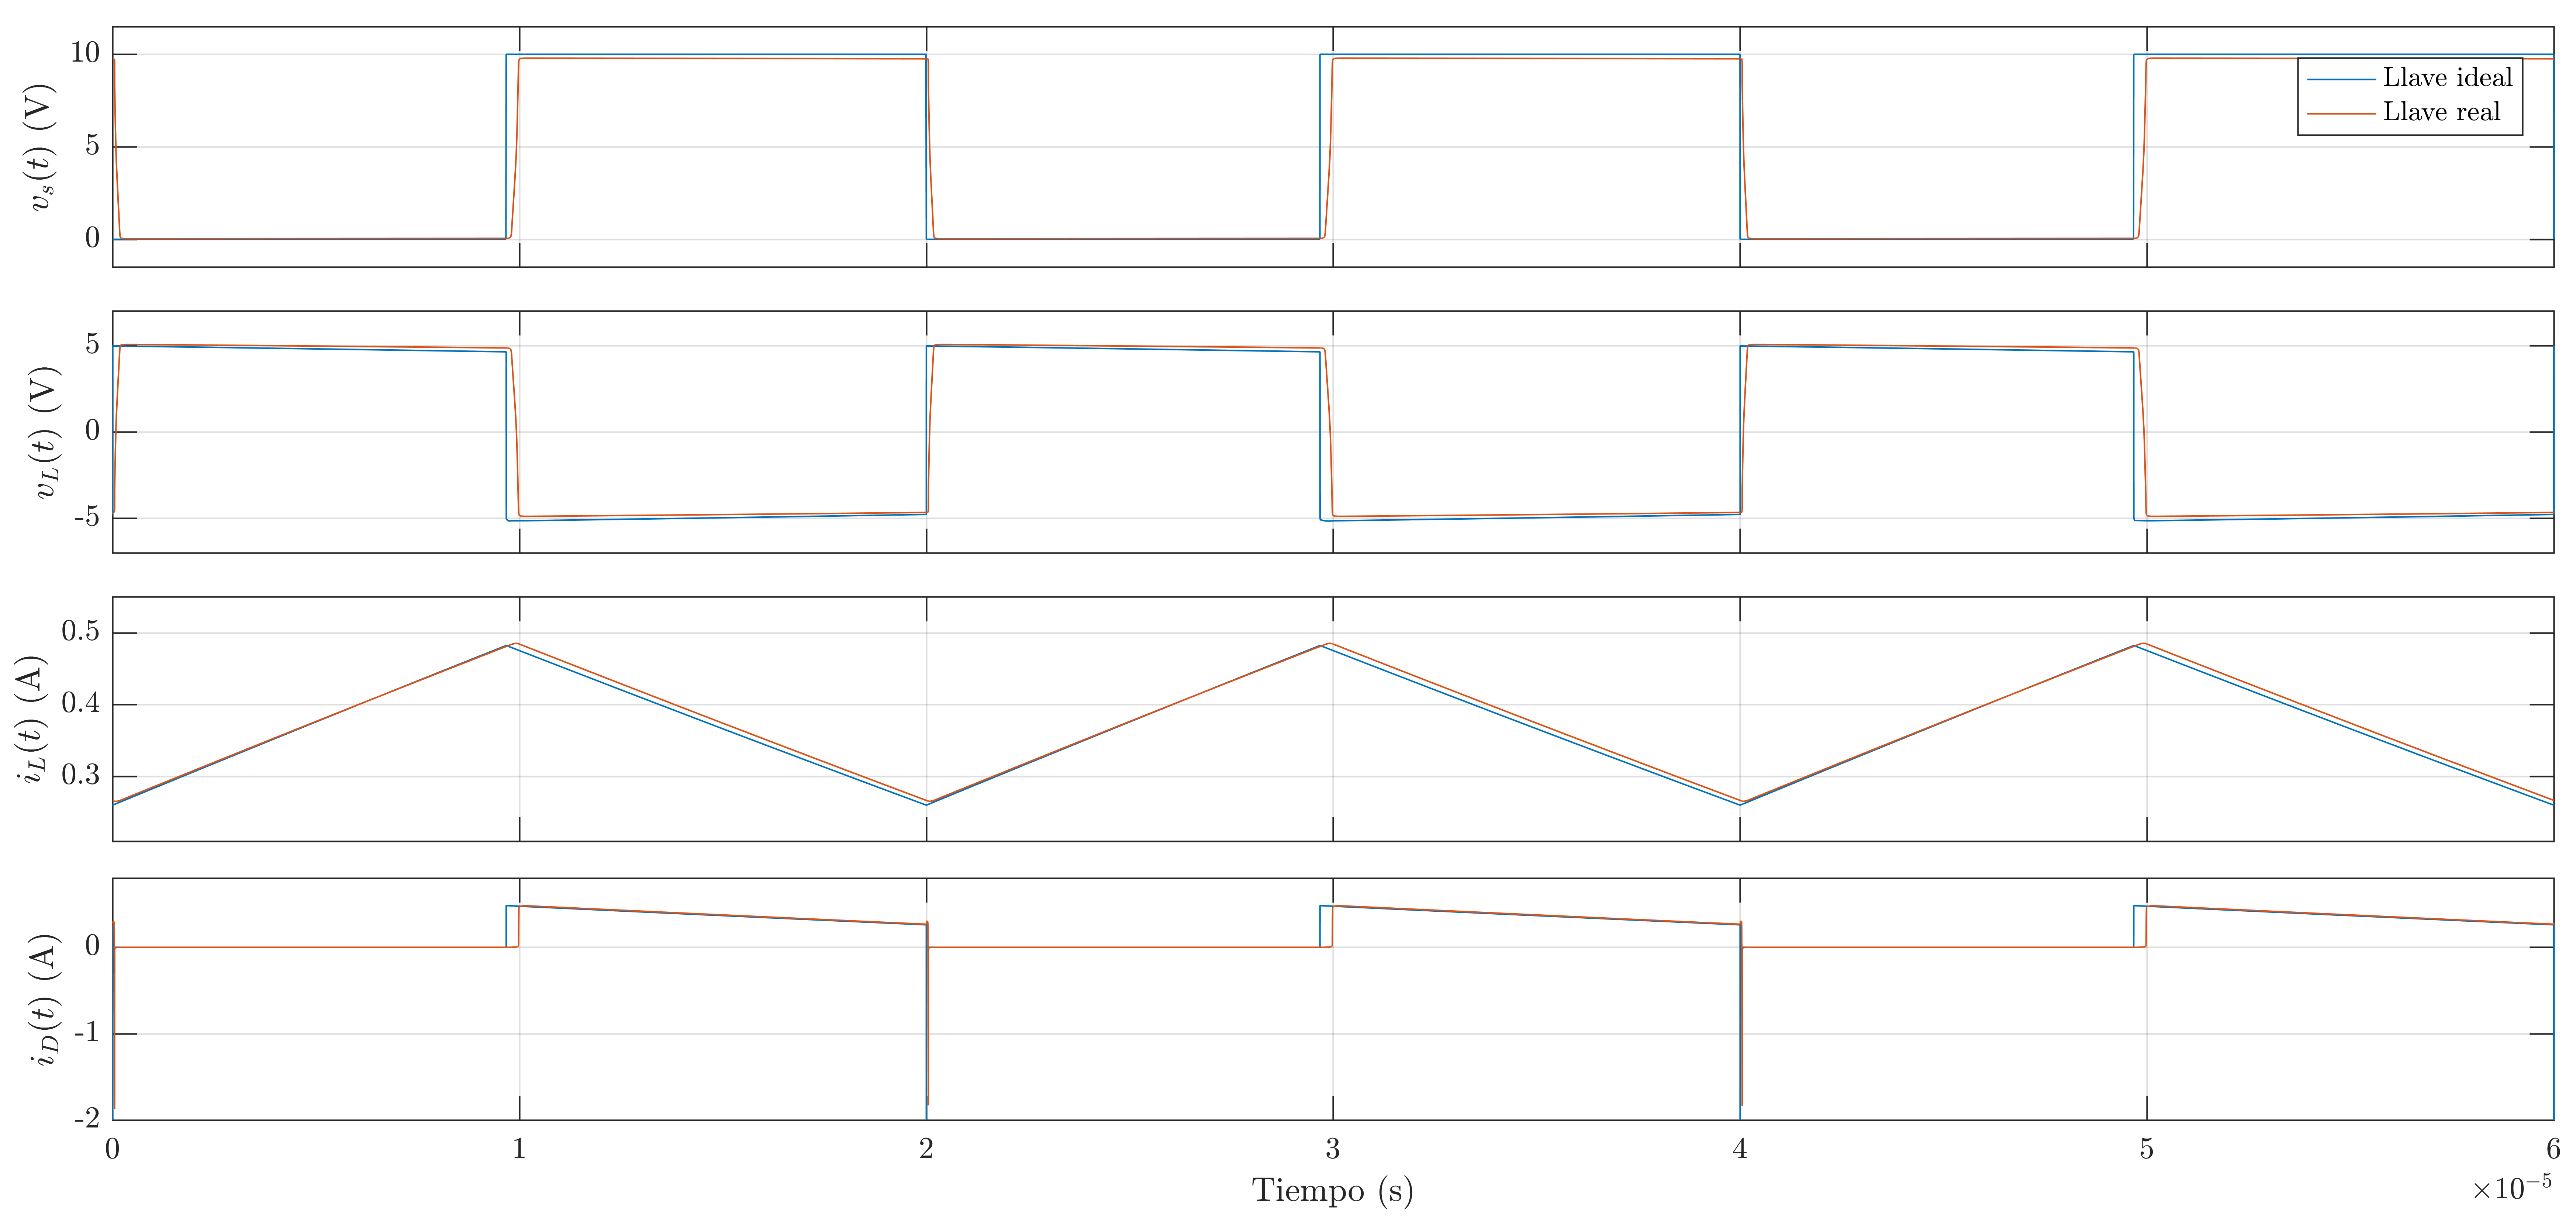
\includegraphics[scale=0.7]{images/ej3/curvas3.png}
		\caption{Curvas simuladas de la fuente buck con llave ideal y con llave real: de arriba hacia abajo, estado de la llave (abierta en 0), tensi\'on en la bobina, corriente en la bobina, y corriente en el diodo.}
		\label{fig:curvas3}
	\end{figure}
	\vspace*{\fill}
\end{landscape}


\end{document}